\documentclass[12pt]{article}
\usepackage[paperwidth=25cm,paperheight=17cm,margin=1.5cm]{geometry}
\usepackage[T1]{fontenc}
\usepackage[utf8]{inputenc}
\usepackage[magyar]{babel}
\usepackage{lmodern}
\usepackage{amsmath}
\usepackage{enumitem}
\usepackage{tikz}
\usetikzlibrary{arrows.meta}

\pagestyle{empty}
\setlength{\parindent}{0pt}
\setlist[enumerate,1]{label=\textbf{\arabic*.}, leftmargin=*, itemsep=5pt, topsep=3pt}
\setlist[enumerate,2]{label=\alph*), leftmargin=2em, itemsep=1pt, topsep=1pt, parsep=0pt}

\begin{document}

\begin{center}\vspace*{-0.4cm}
  {\Large\bfseries Az atom szerkezete -- gyakorló feladatok}\\[4pt]
  \fbox{\parbox{0.94\textwidth}{\centering
    $h = 6{,}63\cdot 10^{-34}~\text{J}\cdot\text{s}$, \;
    $e = 1{,}6\cdot 10^{-19}~\text{C}$, \;
    $m_e = 9{,}1\cdot 10^{-31}~\text{kg}$, \;
    $m_\text{H} = 1{,}67\cdot 10^{-27}~\text{kg}$, \;
    $k = 9\cdot 10^{9}~\tfrac{\text{N}\cdot\text{m}^2}{\text{C}^2}$, \;
    $g = 9{,}8~\tfrac{\text{m}}{\text{s}^2}$, \;
    $hc \approx 1240~\text{eV}\cdot\text{nm}$}}
\end{center}

\begin{minipage}[t]{0.68\linewidth}\vspace{0pt}
\begin{enumerate}
\item \textbf{Fonalsugárcső.} Az $U = 150$~V feszültséggel gyorsított elektronok egy
  ritkított gázzal töltött gömb alakú csőben $B = 0{,}5$~mT indukciójú homogén mágneses
  térben körpályára állnak. A pálya átmérőjét $16{,}6$~cm-nek mérjük.
  \begin{enumerate}
    \item Vezesd le, hogy $\dfrac{e}{m} = \dfrac{2U}{B^2r^2}$, és számold ki a fajlagos
      töltést!
    \item Mekkora az elektronok sebessége?
    \item Hányszor nagyobb az elektron fajlagos töltése, mint a hidrogénioné? Milyen
      következtetést vont le ebből Thomson?
    \item Miért látjuk az elektronnyaláb útját? (Gondolj a Bohr-modellre!)
  \end{enumerate}
\end{enumerate}
\end{minipage}\hfill
\begin{minipage}[t]{0.29\linewidth}\vspace{0pt}\centering
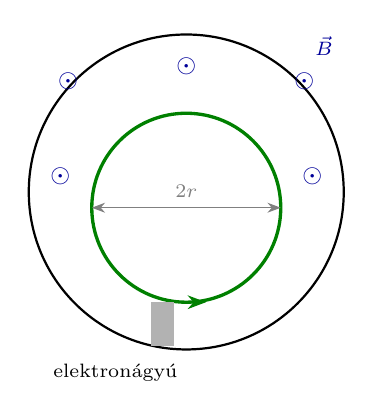
\begin{tikzpicture}[>=Stealth,font=\small]
  \draw[thick] (0,0) circle (2.0);
  \draw[very thick,green!50!black] (0,-0.2) circle (1.2);
  \fill[gray!60] (-0.45,-1.95) rectangle (-0.15,-1.4);
  \node[font=\scriptsize] at (-0.9,-2.3) {elektronágyú};
  \draw[->,thick,green!50!black] (-0.15,-1.4) -- (0.25,-1.4);
  \foreach \x/\y in {-1.5/1.4,0/1.6,1.5/1.4,-1.6/0.2,1.6/0.2}
    \node[blue!60!black] at (\x,\y) {$\odot$};
  \node[blue!60!black,font=\scriptsize] at (1.75,1.85) {$\vec B$};
  \draw[<->,gray] (-1.2,-0.2) -- node[above,font=\scriptsize] {$2r$} (1.2,-0.2);
\end{tikzpicture}
\end{minipage}

\vspace{4pt}
\begin{enumerate}[start=2]
\item \textbf{Millikan kísérlete.} A vízszintes lemezek távolsága $d = 5$~mm.
  \begin{enumerate}
    \item Egy $m = 1{,}63\cdot 10^{-15}$~kg tömegű csepp $U = 250$~V feszültségnél lebeg.
      Mekkora a töltése? Hány elemi töltésnek felel meg?
    \item A csepp negatív töltésű. Melyik lemez a pozitív?
    \item További cseppek mért töltései: $4{,}79$; $8{,}01$; $6{,}42$; $11{,}18$
      ($10^{-19}$~C). Határozd meg ezekből (és az a) részből) az elemi töltés értékét!
    \item Mi történik, ha a lebegő csepp hirtelen elveszít egy elektront? Mekkora
      feszültség kell ezután ahhoz, hogy újra lebegjen?
    \item Az 1.~feladat eredményével együtt mekkora az elektron tömege?
  \end{enumerate}
\end{enumerate}

\newpage
\begin{enumerate}[start=3]
\item \textbf{Rutherford szórási kísérlete.}
  \begin{enumerate}
    \item Mit jósolt a Thomson-modell az aranyfóliára lőtt $\alpha$-részecskék
      eltérülésére, és miért? (Miért nem tudják az elektronok sem jelentősen eltéríteni
      az $\alpha$-részecskét?)
    \item Mit tapasztaltak valójában? Milyen következtetésekre jutott ebből Rutherford?
    \item Miért kellett nagyon vékony fóliát és vákuumot használni?
    \item Egy $5$~MeV mozgási energiájú $\alpha$-részecske (töltése $2e$) egyenesen egy
      aranyatommag ($Z = 79$) felé repül. Milyen közel jut a maghoz, mielőtt
      visszafordul? Mit mond ez a mag méretéről, ha az aranyatom sugara kb.\
      $1{,}4\cdot 10^{-10}$~m?
    \item Miért pattant vissza néhány részecske, és miért csak ilyen kevés?
  \end{enumerate}

\item \textbf{A hidrogénatom színképe.} A hidrogénatom energiaszintjei
  $E_n = -\dfrac{13{,}6~\text{eV}}{n^2}$.
  \begin{enumerate}
    \item Számold ki az első négy szint energiáját, és rajzold fel az energiaszint-ábrát!
    \item Számold ki a $3\to2$, $4\to2$ és $5\to2$ átmenetekben kibocsátott fény
      hullámhosszát! Milyen színűek?
    \item Miért nem látjuk szemmel a hidrogén $n=1$-re végződő átmeneteiben kibocsátott
      fényt?
    \item Mekkora energia kell az alapállapotú hidrogénatom ionizálásához? Mekkora az a
      legnagyobb hullámhossz, amelyik még ionizálni tudja? És ha az atom az $n=2$
      állapotban van?
    \item Mekkora az elektron pályasugara az $n=2$ és az $n=3$ állapotban?
  \end{enumerate}
\end{enumerate}

\newpage
\begin{minipage}[t]{0.60\linewidth}\vspace{0pt}
\begin{enumerate}[start=5]
\item \textbf{Ütközéses gerjesztés.} Az ábra a Franck--Hertz-kísérlet mért görbéje
  higanygőzzel.
  \begin{enumerate}
    \item Miért esik le az áram $4{,}9$~V-nál? Miért ismétlődik ez $4{,}9$~V-onként?
    \item Mekkora hullámhosszú fényt bocsátanak ki a gerjesztett higanyatomok? Látható ez
      a fény?
    \item Milyen görbét várnánk, ha az atom energiája folytonosan változhatna?
    \item Alapállapotú hidrogénatomokat $12{,}5$~eV mozgási energiájú elektronokkal
      bombázunk. Mely állapotokba gerjesztődhetnek az atomok? Milyen hullámhosszú
      vonalak jelennek meg a színképben, és ezek közül melyik látható?
    \item Ha $12{,}5$~eV energiájú \emph{fotonokkal} világítanánk meg ugyanezt a gázt,
      elnyelődnének? Mi a különbség a foton és az elektron között ebből a
      szempontból?
  \end{enumerate}
\end{enumerate}
\end{minipage}\hfill
\begin{minipage}[t]{0.37\linewidth}\vspace{0pt}\centering
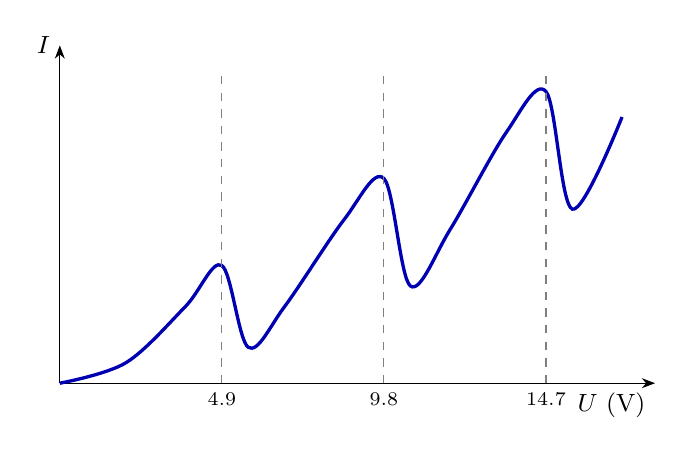
\begin{tikzpicture}[x=0.42cm,y=1.3cm,>=Stealth,font=\small]
  \draw[->] (0,0) -- (18,0) node[below left] {$U$ (V)};
  \draw[->] (0,0) -- (0,3.3) node[left] {$I$};
  \draw[very thick,blue!70!black] plot[smooth,tension=0.55] coordinates {
    (0,0) (2,0.2) (3.8,0.75) (4.9,1.15) (5.7,0.35) (6.8,0.75) (8.6,1.6) (9.8,2.0)
    (10.6,0.95) (11.8,1.5) (13.5,2.45) (14.7,2.85) (15.5,1.7) (17,2.6)};
  \foreach \u in {4.9,9.8,14.7}{
    \draw[gray,dashed] (\u,0) -- (\u,3.0);
    \node[below,font=\scriptsize] at (\u,0) {$\u$};}
\end{tikzpicture}
\end{minipage}

\vspace{6pt}
\begin{enumerate}[start=6]
\item \textbf{De Broglie és Bohr.} A hidrogénatom alapállapotában a pályasugár
  $r_1 = 0{,}053$~nm.
  \begin{enumerate}
    \item Bohr 3.~posztulátuma alapján mekkora az elektron sebessége alapállapotban?
    \item Mekkora ennek az elektronnak a de Broglie-hullámhossza? Hasonlítsd össze a pálya
      kerületével! Hány hullámhossz fér el az $n = 2$ pályán?
    \item Mutasd meg általánosan, hogy a $2\pi r = n\lambda$ állóhullám-feltétel
      ugyanaz, mint Bohr kvantumfeltétele!
    \item Ha az elektron helyét az atom méretén belül, $\Delta x = 0{,}1$~nm pontossággal
      ismerjük, legalább mekkora a sebességének bizonytalansága a Heisenberg-reláció
      szerint? Hasonlítsd össze az a) részben kapott sebességgel! Mit jelent ez a
      ,,pálya'' fogalmára?
  \end{enumerate}

\item \textbf{Szóbeli gyakorlás.} Fejtsd ki összefüggő szövegben, 3--4 percben: \emph{Az
  atommodellek fejlődése.} Minden modellnél térj ki arra, milyen kísérlet vezetett
  hozzá, mit magyarázott meg, és milyen ellentmondás miatt kellett továbblépni!
\end{enumerate}

\end{document}
